\documentclass[11pt]{article}
\usepackage{float}
\usepackage{amsmath}
\usepackage{graphicx}
\usepackage{geometry}
\usepackage[hidelinks]{hyperref}
\usepackage{titlesec}
\usepackage{subcaption}
\usepackage{listings}
\usepackage{xcolor}
\usepackage{algorithm}
\usepackage{algpseudocode}
\usepackage{multirow}

\lstset{
  basicstyle=\ttfamily\footnotesize,
  keywordstyle=\color{blue},
  commentstyle=\color{gray},
  numbers=left,
  numberstyle=\tiny,
  breaklines=true,
  frame=single,
  tabsize=4
}

\geometry{margin=1in}
\titleformat{\section}{\normalfont\Large\bfseries}{\thesection}{1em}{}
\titleformat{\subsection}{\normalfont\large\bfseries}{\thesubsection}{1em}{}

\title{Optimization Techniques: Project}
\author{Maria Charisi 10727}
\date{January 2026\\ 
\href{https://github.com/mariaxarisi/Optimization-Techniques}{\texttt{Github Repo}}}

\begin{document}

\maketitle

\begin{abstract}
This report constitutes the final project for the \textit{Optimization Techniques} course at the \textit{Aristotle University of Thessaloniki}. Its objective is to determine a low-complexity analytic expression, modeled as a linear combination of Gaussians, for a static system described by the unknown nonlinear function $y = f(u_1, u_2)$. A Genetic Algorithm is implemented to optimize the model's parameters, specifically the weights, centers, and widths of the Gaussian components. The study further explores the trade-off between model complexity and accuracy by performing a grid-search hyperparameter tuning for the number of Gaussians, as well as the crossover and mutation probabilities. The proposed solution is rigorously evaluated on a distinct validation dataset, demonstrating the algorithm's ability to effectively reconstruct the underlying system surface with minimal Mean Squared Error (MSE).
\end{abstract}

\tableofcontents
\newpage

\section{Introduction}

This report addresses the problem of identifying an analytic expression for a static system described by the input-output relationship $y = f(u_1, u_2)$ where the internal mathematical structure of $f$ is unknown but continuous. The primary objective is to construct a low-complexity approximation, denoted as $\hat{y}$, using input-output measurements. To achieve this, the system is modeled as a linear combination of $M$ Gaussian functions. The proposed analytic expression takes the following form:

$$\hat{y}(u_1, u_2) = \sum_{i=1}^{M} w_i \cdot G_i(u_1, u_2)$$

where each Gaussian component $G_i$ is defined by its center coordinates $(c_{1,i}, c_{2,i})$ and widths $(\sigma_{1,i}, \sigma_{2,i})$:

$$G_i(u_1, u_2) = e^{- \left[ \frac{(u_1 - c_{1,i})^2}{2\sigma_{1,i}^2} + \frac{(u_2 - c_{2,i})^2}{2\sigma_{2,i}^2} \right]}$$

The challenge lies in determining the optimal set of parameters—specifically the weights $w_i$, centers $c$, and spreads $\sigma$—for all $M$ components to ensure that the model accurately replicates the behavior of the system. To solve this high-dimensional parameter estimation problem, a Genetic Algorithm (GA) is implemented. This evolutionary approach stochastically searches for the optimal configuration by minimizing the error between the model’s predictions and the actual output of the system, avoiding the pitfalls of local minima common in gradient-based methods.

For the purpose of data generation and model evaluation, the underlying system is simulated using the following non-linear function:

$$f(u_1, u_2) = \sin(u_1 + u_2)\sin(u_2^2)$$
% $$u_1 \in [-1, 2]$$
% $$u_2 \in [-2, 1]$$

The inputs are defined within the domains $u_1 \in [-1, 2]$ and $u_2 \in [-2, 1]$. Two distinct datasets were generated to ensure robust testing: a \textit{Training Set} consisting of 300 random samples used to guide the Genetic Algorithm, and a separate \textit{Validation Set} of 150 samples used exclusively to evaluate the performance of the final analytic expression on unseen data. The spatial distribution of the training data samples is illustrated in Figure~\ref{fig:train_data}.

\begin{figure}[H]
    \centering
    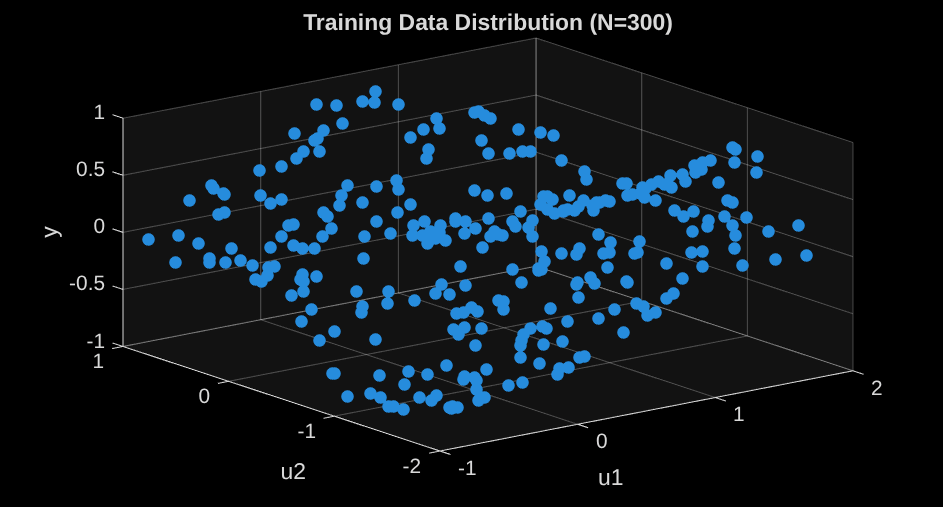
\includegraphics[width=0.75\linewidth]{assets/train_data.png}
    \caption{Training data distribution.}
    \label{fig:train_data}
\end{figure}

\section{Genetic Algorithm}

Genetic Algorithms (GAs) are population-based stochastic optimization methods inspired by the principles of natural selection and genetics. They are particularly well suited for solving complex, non-linear, and non-convex optimization problems, as they do not require gradient information and are less prone to becoming trapped in local optima.

In a standard GA, a candidate solution is represented as a \textit{chromosome}, and its effectiveness is measured by a \textit{fitness function}. For the specific problem, since the model consists of a linear combination of $M$ Gaussian functions, and each Gaussian requires 5 parameters (one weight $w$, two centers $c_1, c_2$, and two widths $\sigma_1, \sigma_2$), the chromosome is constructed as a concatenated vector of $5 \times M$ real numbers.

$$\mathbf{C} = [ \underbrace{w_1, c_{1,1}, \sigma_{1,1}, c_{2,1}, \sigma_{2,1}}_{\text{Gaussian 1}}, \dots, \underbrace{w_M, c_{1,M}, \sigma_{1,M}, c_{2,M}, \sigma_{2,M}}_{\text{Gaussian M}} ]$$

The genetic algorithm starts by initializing a population of candidate solutions with random values drawn within the prescribed parameter bounds. At each generation, individuals are evaluated according to their prediction error, measured by the mean squared error (MSE). Based on these fitness values, the most suitable individuals are selected to produce offspring through arithmetic crossover and mutation operators. This evolutionary process is repeated for a fixed number of generations. The overall procedure is summarized in Algorithm~\ref{algo:ga}.

\begin{algorithm}[H]
\caption{Genetic Algorithm for Function Approximation}
\label{algo:ga}
\begin{algorithmic}[1]
\Require Training Data $(u_1, u_2, y)$, Parameters ($N_{pop}, N_{gen}, p_c, p_m$)
\Ensure Best Solution $\mathbf{x}^*$ (Parameters minimizing MSE)

\State Initialize population $P$ with random real values within bounds
\State $\mathbf{x}_{best} \gets \infty$

\For{$gen = 1$ to $N_{gen}$}
    \State Compute Fitness scores for $P$ based on MSE
    \State $\mathbf{x}_{current\_best} \gets$ Best individual in current $P$
    
    \If{Fitness($\mathbf{x}_{current\_best}$) $>$ Fitness($\mathbf{x}_{best}$)}
        \State $\mathbf{x}_{best} \gets \mathbf{x}_{current\_best}$
    \EndIf
    
    \State $Parents \gets$ Selection($P$) \Comment{Roulette Wheel}
    \State $Offspring \gets$ Crossover($Parents, p_c$) \Comment{Arithmetic Crossover}
    \State $Offspring \gets$ Mutation($Offspring, p_m$) \Comment{Gaussian Mutation}
    
    \State $Offspring[1] \gets \mathbf{x}_{best}$ \Comment{Apply Elitism}
    \State $P \gets Offspring$
\EndFor

\State \Return $\mathbf{x}_{best}$
\end{algorithmic}
\end{algorithm}

\subsection{Initialization}

The optimization process begins with the initialization of a population of candidate solutions $N_{pop}$. Since the problem variables are continuous, a real-valued encoding is employed. The population is represented as a matrix of size $N_{pop} \times (5M)$, where each row corresponds to a single chromosome vector. The genes are initialized uniformly at random within specific domain constraints to ensure the search begins in a feasible region of the solution space:

\begin{itemize}
\item \textbf{Weights ($w_i$):} Initialized in the range $[-10, 10]$.
\item \textbf{Centers ($c_{1,i}, c_{2,i}$):} Constrained to the input domains $[-1, 2]$ and $[-2, 1]$ respectively.
\item \textbf{Widths ($\sigma_{1,i}, \sigma_{2,i}$):} Initialized within $[0.2, 1.5]$ to avoid singularities or overly flat basis functions.
\end{itemize}

\subsection{Fitness Evaluation}

The quality of each individual is determined by how accurately its corresponding Gaussian model approximates the training data. For a given chromosome, the predicted output $\hat{y}$ is computed for all training inputs by reconstructing the linear combination of Gaussians. The objective is to minimize the Mean Squared Error (MSE) between the predicted output and the true system output $y$:

$$MSE = \frac{1}{N} \sum_{k=1}^{N} (y_k - \hat{y}_k)^2$$

where $N$ is the number of training samples. To convert this minimization problem into a maximization problem suitable for the selection mechanism, the fitness function is defined as:

$$Fitness(\mathbf{x}) = \frac{1}{1 + MSE(\mathbf{x})}$$

This transformation normalizes the score, ensuring that individuals with lower error receive higher fitness values approaching 1.

\subsection{Selection}

To drive the evolutionary process, parents are selected from the current population based on their fitness values. At each generation, a total of $N_{pop}$ individuals are selected to form the mating pool for reproduction. The selection mechanism employed is Roulette Wheel Selection enhanced with Linear Dynamic Scaling.

Standard roulette wheel selection can suffer from scaling issues: in early generations, a highly fit individual may dominate the population, leading to premature convergence, while in later generations, diminishing fitness differences may result in stagnation. To alleviate these effects, the raw fitness values are linearly scaled to the interval $[0,1]$ prior to selection:

$$
Fitness^{scaled}_i = \frac{Fitness_i - Fitness_{min}}{Fitness_{max} - Fitness_{min}} + \epsilon
$$

where $Fitness_{min}$ and $Fitness_{max}$ denote the minimum and maximum fitness values in the current population, respectively, and $\epsilon$ is a small positive constant introduced to avoid division by zero.

Selection probabilities are then computed based on the scaled fitness values. Specifically, the probability $P_i$ of selecting the $i$-th individual is given by:

$$
P_i = \frac{Fitness^{scaled}_i}{\sum_{j=1}^{N_{pop}} Fitness^{scaled}_j}
$$

Using these probabilities, $N_{pop}$ individuals are stochastically selected with replacement to form the parent population, ensuring that individuals with higher fitness have a proportionally greater chance of contributing to the next generation while maintaining population diversity.

\subsection{Crossover}

The crossover operator promotes exploration of the search space by recombining genetic material from selected parent solutions. In this work, Arithmetic Crossover is employed, which is well suited for real-coded chromosomes. Given two selected parents $\mathbf{P}_1$ and $\mathbf{P}_2$, two offspring $\mathbf{O}_1$ and $\mathbf{O}_2$ are generated with probability $p_c$ according to:

$$ \mathbf{O}_1 = \alpha \cdot \mathbf{P}_1 + (1-\alpha) \cdot \mathbf{P}_2 $$
$$ \mathbf{O}_2 = \alpha \cdot \mathbf{P}_2 + (1-\alpha) \cdot \mathbf{P}_1 $$

where $\alpha$ is a weighting coefficient sampled from a uniform distribution $\mathcal{U}(0,1)$. With probability $1 - p_c$, no crossover is performed and the offspring are exact copies of the parents. This operator generates new candidate solutions that lie on the line segment connecting the parent solutions, thereby exploiting the convex region between high-quality individuals.

\subsection{Mutation}

To preserve genetic diversity and reduce the risk of premature convergence to local optima, Gaussian mutation is applied to the offspring population. Each gene of an offspring chromosome is independently mutated with probability $p_m$. When mutation occurs, a random noise sampled from a zero-mean normal distribution is added to the gene value:

$$
x_{new} = x_{old} + \mathcal{N}(0, \sigma_{noise}^2)
$$

Following mutation, boundary constraints are enforced to ensure feasibility of the solutions. If a mutated gene violates its predefined parameter bounds, it is clipped to the nearest valid boundary. This guarantees that all individuals remain physically meaningful throughout the evolutionary process.

\subsection{Elitism}

To ensure that the best solution found is not lost due to stochastic genetic operations, an elitism strategy is employed. Specifically, the single best individual identified across all generations is preserved and directly copied into the next generation, replacing the first individual of the new population. This mechanism guarantees a non-decreasing best fitness value over successive generations.

\section{Parameter Tuning}

The performance of the Genetic Algorithm and the quality of the resulting approximation model are highly sensitive to the choice of hyperparameters. These parameters control the algorithm's population dynamics, exploration-exploitation trade-off, and the complexity of the final model. 

The hyperparameters can be categorized into two groups: those related to the GA's evolutionary process (population size, generations, probabilities) and those defining the search space of the Gaussian model (parameter ranges, number of Gaussians). A baseline configuration was established based on preliminary experiments and literature recommendations, as summarized in Table~\ref{tab:baseline_params}.

\begin{table}[H]
\centering
\caption{Baseline Parameter Configuration}
\label{tab:baseline_params}
\begin{tabular}{llc}
\hline
\textbf{Category} & \textbf{Parameter} & \textbf{Value} \\ \hline
\multirow{5}*{GA Settings} 
 & Population Size ($N_{pop}$) & 100 \\
 & Max Generations ($N_{gen}$) & 3000 \\
 & Crossover Probability ($p_c$) & \textit{Tuned} \\
 & Mutation Probability ($p_m$) & \textit{Tuned} \\
 & Mutation Noise ($\sigma_{noise}$) & 0.1 \\ \hline
\multirow{5}*{Model Constraints} 
 & Number of Gaussians ($M$) & \textit{Tuned} \\
 & Center 1 Range ($c_1$) & $[-1, 2]$ \\
 & Center 2 Range ($c_2$) & $[-2, 1]$ \\
 & Weight Range ($w$) & $[-10, 10]$ \\
 & Width Range ($\sigma$) & $[0.2, 1.5]$ \\ \hline
\end{tabular}
\end{table}

To determine the optimal configuration, a tuning process was conducted for three critical parameters: the number of Gaussian components ($M$), the crossover probability ($p_c$), and the mutation probability ($p_m$). The selection criterion for all tuning experiments was the minimization of the Mean Squared Error (MSE) on the independent \textit{Validation Set}.

\subsection{Number of Gaussians}

The number of Gaussian basis functions, $M$, impact directly the complexity of the model. A model with too few Gaussians may fail to capture the underlying system dynamics, while an excessive number may lead to overfitting the training data and poor generalization.

To find the optimal balance, a search was performed by varying $M$ from 2 to 15. For each value of $M$, the GA was executed, and the best solution's performance was evaluated on the validation set. The relationship between model complexity and validation error is presented in Figure~\ref{fig:tuning_complexity}.

\begin{figure}[H]
    \centering
    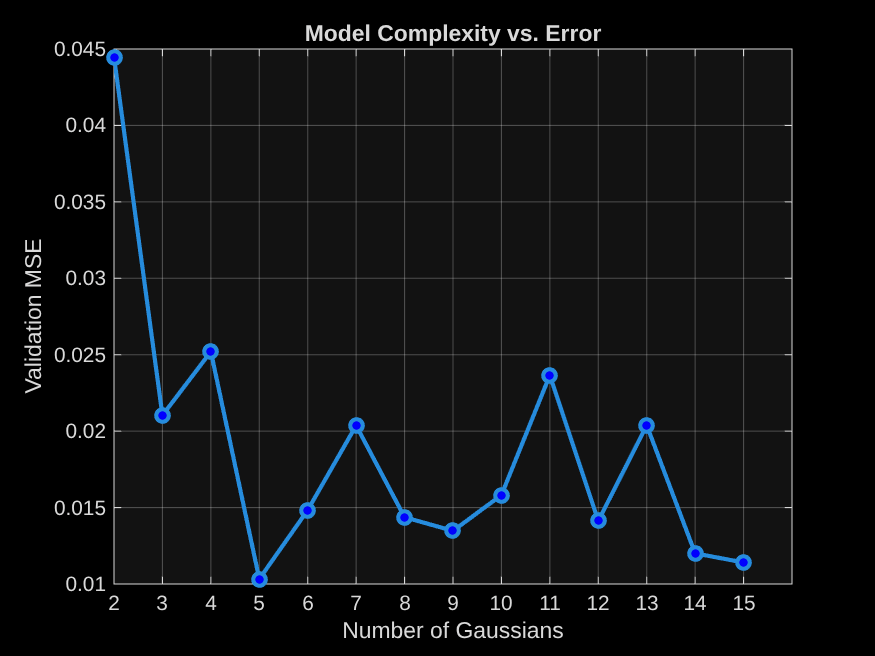
\includegraphics[width=0.7\linewidth]{assets/tuning_complexity.png}
    \caption{Validation MSE versus the number of Gaussian components ($M$).}
    \label{fig:tuning_complexity}
\end{figure}

As observed in the figure, the validation error initially decreases rapidly as complexity increases, indicating that additional model capacity is needed to capture the function's behavior. The error reaches a minimum at $M=5$ Gaussians. Beyond this point, adding more Gaussians does not yield significant improvements and, in some cases, leads to a slight increase in validation error, suggesting the onset of overfitting. Consequently, $M=5$ was selected as the optimal model complexity for the final solution.

\subsection{Crossover and Mutation Probabilities}

The crossover ($p_c$) and mutation ($p_m$) probabilities are critical for balancing exploration (searching new regions of the space) and exploitation (refining existing good solutions). To find the optimal combination, a grid search was performed over the following ranges:
\begin{itemize}
    \item \textbf{Crossover Probability ($p_c$):} $\{0.5, 0.6, 0.7, 0.8, 0.9\}$
    \item \textbf{Mutation Probability ($p_m$):} $\{0.05, 0.10, 0.15, 0.20, 0.25\}$
\end{itemize}

This resulted in a total of $25$ different hyperparameter configurations. The GA was run for each combination, and the resulting validation MSE was recorded. The results of this grid search are visualized in the heatmap shown in Figure~\ref{fig:tuning_heatmap}.

\begin{figure}[H]
    \centering
    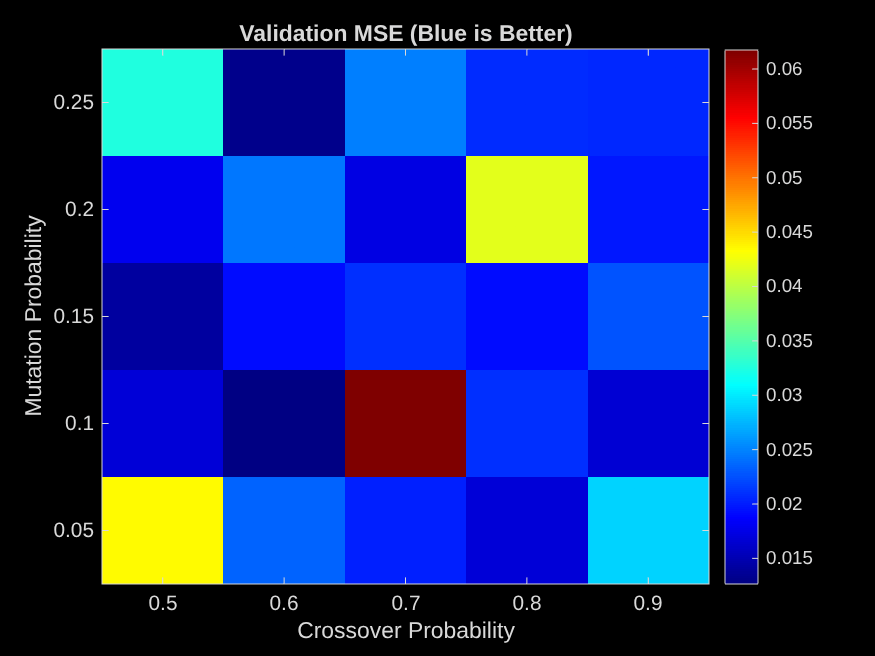
\includegraphics[width=0.7\linewidth]{assets/tuning_heatmap.png}
    \caption{Heatmap of Validation MSE for different combinations of crossover and mutation probabilities. Dark blue indicates lower error.}
    \label{fig:tuning_heatmap}
\end{figure}

The global minimum validation MSE was achieved with the combination of $p_c = 0.6$ and $p_m = 0.1$. These values were selected for the final execution of the Genetic Algorithm.

\newpage
\section{Results}

Following parameter tuning, the Genetic Algorithm was executed using the baseline configuration and the selected optimal hyperparameters: $M=5$ Gaussian components, a crossover probability of $p_c = 0.6$, and a mutation probability of $p_m = 0.1$. The algorithm was run for $N_{gen}=3000$ generations with a population size of $N_{pop}=100$.

\subsection{MSE Performance}

The best solution obtained at the end of the process was evaluated on both the \textit{Training Set} (used during optimization) and the distinct \textit{Validation Set} (unseen data). The final Mean Squared Error (MSE) metrics are presented in Table~\ref{tab:final_results}.

\begin{table}[H]
\centering
\caption{Final Performance Metrics of the Optimized Gaussian Model}
\label{tab:final_results}
\begin{tabular}{lc}
\hline
\textbf{Dataset} & \textbf{Mean Squared Error (MSE)} \\ \hline
Training Set (300 samples) & $0.005893$ \\
Validation Set (150 samples) & $0.006183$ \\ \hline
\end{tabular}
\end{table}

The results show high accuracy, with MSE values on the order of $10^{-3}$. The close agreement between training and validation errors, differing by only $0.00029$, indicates strong generalization and confirms that the model does not overfit, supporting the choice of $M=5$ Gaussians.

\subsection{Convergence Analysis}

The evolutionary history of the best solution's fitness over the 3000 generations is illustrated in Figure~\ref{fig:convergence}. The plot shows the MSE of the best individual on the training set at each generation on a logarithmic scale.

\begin{figure}[H]
    \centering
    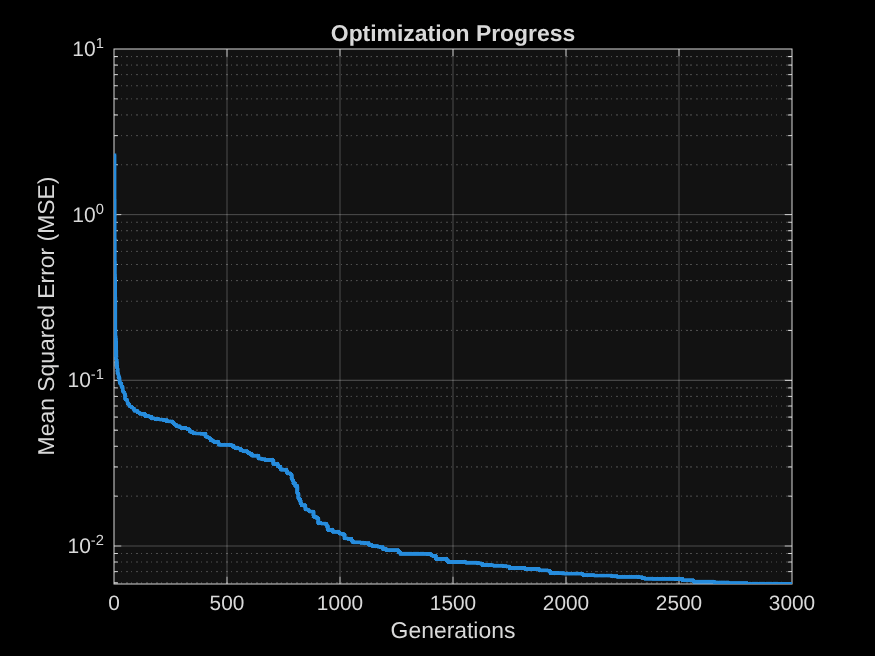
\includegraphics[width=0.7\linewidth]{assets/mse_convergence.png}
    \caption{Convergence history of the Genetic Algorithm.}
    \label{fig:convergence}
\end{figure}

The convergence behavior exhibits typical GA characteristics. In the initial generations (approximately 0 to 1000), there is a rapid decrease in error as the algorithm explores the search space and identifies promising regions. Subsequently, the process enters a refinement phase, characterized by a slower, monotonic decrease in MSE as mutation exploit the identified basin of attraction. The presence of elitism ensures the curve never increases, providing stable convergence toward the final solution.

\subsection{Visual Comparison}

To evaluate the model's performance, the surface generated by the final analytic expression $\hat{y}(u_1, u_2)$ is compared directly against the true system surface $y=f(u_1, u_2)$ over the entire input domain. This comparison is presented in Figure~\ref{fig:surface_comparison}.

\begin{figure}[H]
    \centering
    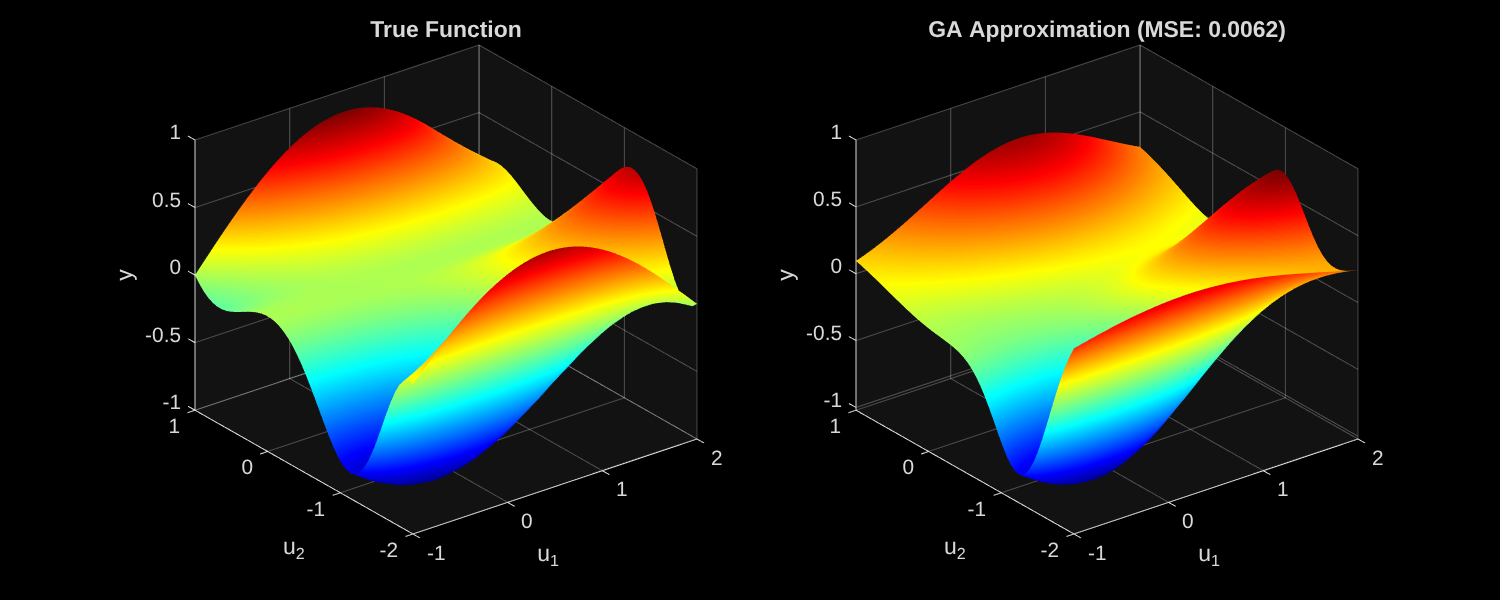
\includegraphics[width=\linewidth]{assets/comparison.png}
    \caption{Visual comparison of the system surfaces. Left: The ground truth function $f(u_1, u_2)$. Right: The approximation $\hat{y}(u_1, u_2)$ generated by the GA-optimized model with $M=5$ Gaussians.}
    \label{fig:surface_comparison}
\end{figure}

The approximated surface successfully captures the major topographical features of the true function, including the locations and magnitudes of the primary peaks and valleys. The smooth nature of the Gaussian basis functions results in a clean approximation that accurately models the underlying non-linear relationship without capturing noise or exhibiting high-frequency oscillations.

\end{document}
